\documentclass[11pt]{article}

% Change "review" to "final" to generate the final (sometimes called camera-ready) version.
% Change to "preprint" to generate a non-anonymous version with page numbers.
\usepackage[final]{acl}

% Standard package includes
\usepackage{times}
\usepackage{latexsym}

% For mathematical typesetting and \text command
\usepackage{amsmath}

% For customizing lists (enumerate, itemize)
\usepackage{enumitem}

% tu use algorithms 
\usepackage{algorithm}
\usepackage{algpseudocode}
\usepackage{xcolor}

% For proper rendering and hyphenation of words containing Latin characters (including in bib files)
\usepackage[T1]{fontenc}
% For Vietnamese characters
% \usepackage[T5]{fontenc}
% See https://www.latex-project.org/help/documentation/encguide.pdf for other character sets

% This assumes your files are encoded as UTF8
\usepackage[utf8]{inputenc}

% For cross-references with \cref command
\usepackage{cleveref}

% This is not strictly necessary, and may be commented out,
% but it will improve the layout of the manuscript,
% and will typically save some space.
\usepackage{microtype}

% This is also not strictly necessary, and may be commented out.
% However, it will improve the aesthetics of text in
% the typewriter font.
\usepackage{inconsolata}

%Including images in your LaTeX document requires adding
%additional package(s)
\usepackage{graphicx}
\usepackage{booktabs}
\usepackage{multirow}

% If the title and author information does not fit in the area allocated, uncomment the following
%
%\setlength\titlebox{<dim>}
%
% and set <dim> to something 5cm or larger.

\title{FastDetectGPT: Understanding Sampling-based Zero-shot AI-generated Text Detection}

\author{
  \textbf{Jose Garcia\textsuperscript{1}},
  \textbf{Krystof Bobek\textsuperscript{1}},
  \textbf{Mara Dragomir\textsuperscript{1}}, \\
  \textbf{Mahdi Rahimi\textsuperscript{1}},
  \textbf{Salvador Torpes\textsuperscript{1}}
\\
\\
  \textsuperscript{1}University of Amsterdam
\\
\\
  \textbf{Contact:} \{
    \texttt{jose.garcia.carrillo, krystof.bobek, mara.dragomir,} \\
    \texttt{mahdi.rahimi, salvador.baptista.torpes} \}
    \texttt{@student.uva.nl}
}

\begin{document}

\maketitle

\begin{abstract}
  DetectGPT introduced a zero-shot, sampling-based method for detecting machine-generated text by exploiting the local curvature of a model's log-likelihood function. Fast-DetectGPT later improved this method, matching performance at far lower cost. In this work, we reproduce Fast-DetectGPT and extend evaluation to new source models (DeepSeek R1 Distill Llama, Microsoft Phi 2, Mistral 7B, GPT-4o mini). We assess performance on three datasets: XSum, HC3, and Scottish Gaelic from XL-Sum as an under-represented language. Additionally, we propose a novel adversarial setting: the Mid-K perturbation attack, which forces the generator to avoid high-probability tokens at random positions during decoding. Our results show that Fast-DetectGPT remains highly effective and can generalize well across diverse models, datasets, and languages, but that decoding perturbations reduce its accuracy, revealing a key vulnerability. The original code and our extensions are available on GitHub: \url{https://github.com/salvatorpes/zero-shot-llm-detection}.
\end{abstract}


\section{Introduction}

Large language models (LLMs) such as ChatGPT \cite{GPT3}, have transformed content creation in journalism, education, and research. However, their fluency raises concerns about misuse, especially in the generation of fake news \cite{ahmed2021detectingfakenewsusing}, fraudulent reviews \cite{adelani2019generatingsentimentpreservingfakeonline}, and plagiarism \cite{Lee_2023}. As these models become increasingly better, distinguishing machine- from human-written text is difficult even for experts \cite{shahid2022areyouacyborg}, highlighting the need for reliable automated detection methods.

Detection approaches fall into two groups: \textit{supervised classifiers} and \textit{zero-shot methods}. Supervised detectors rely on fine-tuning language models with labeled human and machine-written examples to learn distinguishing patterns \cite{mitrovic2023chatgpthumandetectexplain}. Although effective within their training domains, such models tend to generalize poorly to unseen models or domains \cite{bakhtin2019realfakelearningdiscriminate}. In contrast, zero-shot methods \cite{su2023detectllm} leverage pre-trained language models without additional training, relying on generalizable statistical or probabilistic clues instead. This makes them more robust to domain and model variations.

Zero-shot detectors operate by identifying intrinsic statistical properties of text, such as word ranking, token likelihood, and entropy. The key assumption is that machine-generated and human-written texts show different statistical properties. For example, LLMs typically assign higher log-likelihoods to their own outputs than to human-written passages, as they favour more probable sequences and tokens during decoding. Therefore, by designing algorithms that measure internal text properties and compare them against a threshold, we can classify them as machine-generated or human-written.


\section{Methodology}\label{sec:methodology}

We frame detection as \textit{zero-shot binary classification}: given a candidate passage, determine whether it was written by a human or generated by a language model. We build on DetectGPT and Fast-DetectGPT, extending to new models, datasets, and introducing a novel adversarial attack.

\subsection{Methods}

Baseline methods compare internal model properties against a threshold to decide if text is human- or machine-generated.

DetectGPT \cite{detectgpt} introduced a sampling-based criterion for detection. Its central hypothesis is that model-generated text variations tend to exhibit lower log-probabilities than the original, placing them in regions of negative curvature within the source model’s log-likelihood function. DetectGPT generates multiple perturbations of a candidate passage using a masked language model (e.g., T5), then scores both the original and its perturbations with the source model. If the original scores higher than its perturbations, it is likely machine-generated; otherwise human-written. While effective, this method is computationally expensive, as it requires scoring a large number of perturbations per passage (often more than 100).

Fast-DetectGPT replaces DetectGPT’s perturb-and-score pipeline with a single-pass estimate of the conditional probability curvature. Framed as a sequential token selection problem, the hypothesis is that language models approximate the modal human distribution, favouring safer, higher-probability tokens, whereas individuals choose more diverse words. Consequently, model-generated text tends to lie near local maxima of the conditional probability function (positive curvature), while human text remains closer to flat regions (curvature near zero). 

Operationally, Fast-DetectGPT samples alternative token choices independently at each position (conditioned on the observed prefix), computes their conditional probabilities under a scoring model, and aggregates these into a curvature statistic. All alternatives are produced once and scored in a single batch, avoiding per-perturbation scoring. Accuracy matches DetectGPT with far better efficiency.
% \vspace{-1em}
\begin{equation}
  (\log p_\theta (x)-\tilde{\mu})/\tilde{\sigma} > \epsilon \rightarrow x \text{ is machine} 
  \label{eq:fastdetect}
\end{equation}

In \cref{eq:fastdetect}, $x$ is the candidate passage. $q_\varphi(\tilde{x}|x)$ is the sampling model , $p_\theta$ is the scoring model, $\tilde{\mu}$ and $\tilde{\sigma}$ are the sample mean and standard deviation of the perturbations log-probabilities under $p_\theta$, and $\epsilon$ is a tunable threshold. The passage $x$ is classified as machine-generated if its standardized log-probability exceeds $\epsilon$. This formulation is also valid for DetectGPT when $q_\varphi(\tilde{x}|x)$ corresponds to its perturbation distribution. The pseudocode for both algorithms is presented in \cref{alg:fastdetectgpt} and \cref{alg:detectgpt}.

\subsection{Models}

Fast-DetectGPT employs three main model components: the source model, which generates candidate text by conditioning on a human-written prefix (first 30 tokens) and decoding from it; the sampling model which produces conditional token distributions used to generate perturbations $\tilde{x}_i$ of each candidate passage $x$; and the scoring model scores log-probabilities.
% \begin{enumerate}[leftmargin=*]
%   \item \textbf{Source model}: Generates candidate text by conditioning on a human-written prefix (first 30 tokens) and decoding from it.
%   \item \textbf{Sampling model} ($q_\varphi$): Produces conditional token distributions used to generate perturbations $\tilde{x}_i$ of each candidate passage $x$.
%   \item \textbf{Scoring model} ($p_\theta$): Computes log-probabilities for evaluating the perturbed sequences.
% \end{enumerate}

Detection experiments are conducted under two configurations:
\textit{white-box} (where source and scoring models are identical) and \textit{black-box} (a more realistic setting). %The sampling model may differ from the scoring model in both cases, which can sometimes enhance detection robustness when they are not the same.

\subsection{Datasets}

The models are evaluated on synthetic datasets created by prompting the source with the first 30 human tokens. The model then generates continuations up to an average of 230 total tokens, producing the necessary machine-generated text samples.

We use two human-written datasets to construct these new synthetic ones:
XSum \cite{XSum}, a large collection of documents and their summaries, and HC3 \cite{HC3}, a dataset of human and GPT-3.5-generated answers to the same questions (using only the human responses). From each, up to 500 human texts generate corresponding synthetic continuations.

\subsection{Mid-K Attack}

To evaluate detector robustness, we introduce the Mid-K Attack, a perturbation strategy that alters the token selection process during generation. At a fixed number of randomly selected positions, the top-$K$ most probable tokens in the model’s next-token distribution are banned (logits set to $-\infty$), forcing sampling from lower-probability tokens.

Mid-K has three parameters: $P$ (the number of positions per sequence where the ban is applied), $K$ (number of top tokens excluded at each position), and $S$ (the first generated-token index eligible for perturbation).
% \begin{itemize}[leftmargin=*]
%   \item $P$: number of positions per sequence where the ban is applied,
%   \item $K$: number of top tokens excluded at each position,
%   \item $S$ (optional): the first generated-token index eligible for perturbation (useful to avoid modifying early tokens).
% \end{itemize}

For each sequence, we compute the maximum number of generated tokens $M = \texttt{max\_length} - \texttt{prompt\_length}$ and select up to $P$ positions from $\{S, \ldots, M\}$. At each chosen position, we set the top-$K$ logits to $-\infty$ and sample from the remaining options.


\section{Experiments}

Our experiments evaluate Fast-DetectGPT’s performance and robustness against three baseline methods from the original study (Likelihood, Entropy, and LogRank), across architectures, datasets, and adversarial settings. We report AUROC and run all experiments in the \textit{white-box} setting. DetectGPT was run only once due to computational limits (see Table~\ref{tab:main_results}).

\subsection{Reproducibility Study}

We first assess the reproducibility and generalization of Fast-DetectGPT across different model architectures and datasets. We chose three small open-weight models of varying sizes: DeepSeek R1 Distill Llama 8B \cite{deepseekai}, Microsoft Phi-2 (2.7B parameters) \cite{phi2}, and Mistral 7B Instruct v0.2 \cite{mistral}. These models were evaluated on the datasets mentioned above, XSum and HC3.  This tests stability across domains, lengths, formats, and model sizes.

\subsection{Closed-Weight API Model}

To further test the method’s applicability, in addition to the three open-weight models, we evaluate Fast-DetectGPT on a closed-weight API model: GPT-4o mini. Unlike open-weight models, GPT-4o mini only gives access to the top-20 token probabilities per token. While this limitation prevents a direct comparison with the open-weight models, the goal of this experiment is to analyze how restricted access to token probabilities affects detection performance.

\subsection{Low-Resource Language}

We also investigate Fast-DetectGPT’s robustness in low-resource language settings. For this, we employ the XL-Sum dataset \cite{xlsum}, an extension of XSum covering multiple languages, and focus on the Scottish Gaelic subset. This experiment aims to determine whether Fast-DetectGPT can maintain detection accuracy when applied to languages with limited pre-training data and distinctive linguistic characteristics.

\subsection{Adversarial Attack}

Finally, we evaluate the robustness of all detectors under the Mid-K adversarial attack introduced in Section~\ref{sec:methodology}. The objective is to quantify how detection accuracy degrades as attack strength increases.

%\textit{Setup.}  
We conduct all adversarial experiments using the GPT-2 model on the XSum dataset, since the goal is to analyze the impact of Mid-K parameters rather than variations in models or datasets, and since we had to consider computational limitations. For each example, the generator is prompted with the first 30 tokens and produces a continuation of up to 200 tokens. The Mid-K attack is applied during decoding, while the detection pipeline (Fast-DetectGPT) remains unchanged, ensuring that any observed performance degradation is attributable only to the attack.

% Should we cite GPT 2? and mention if it was used in the original study

%\textit{Parameter grid.}  
We explore the following parameter ranges: $P \in \{1,5,10,20,30,50,60,70,80,90,100,150\}$,  $K \in \{1,2,5,10,20\}$, and fixed $S=5$. Each $(P, K)$ pair corresponds to one experiment, where Mid-K is applied at up to $P$ positions starting from token index $S$. In total, 60 parameter combinations are tested, covering a wide spectrum of perturbation strengths.

%\textit{Scope.}  
% Since the goal is to analyze the impact of Mid-K parameters rather than variations in models or datasets, and since we had to consider computational limitations, all adversarial experiments are restricted to this single model–dataset configuration.

\begin{table}[h]
    \centering
    \small
    \begin{tabular}{l|ccc|c}
    \toprule
    \multirow{2}{*}{\textbf{Method}} & \multicolumn{4}{c}{XSum} \\
    \cmidrule{2-5}
    & \textbf{R1-8B} & \textbf{Phi-2} & \textbf{Mistral} & \textbf{Avg.} \\
    \midrule
    Likelihood & 0.9999 & 0.8782 & 0.9665 & 0.9482 \\
    Entropy & 0.1645 & 0.5411 & 0.4558 &  0.3871\\
    LogRank & \textbf{1.0000} & 0.9051 & 0.9596 & 0.9549 \\
    \midrule
    DetectGPT & 0.8560 & - & - & - \\
    Fast-DetectGPT & \textbf{1.0000} & \textbf{0.9769} & \textbf{0.9989} & \textbf{0.9919} \\
    \bottomrule
    \end{tabular}
    \vspace{0.5em}
    
    \begin{tabular}{l|ccc|c}
    \toprule
    \multirow{2}{*}{\textbf{Method}} & \multicolumn{4}{c}{HC3} \\
    \cmidrule{2-5}
    & \textbf{R1-8B} & \textbf{Phi-2} & \textbf{Mistral} & \textbf{Avg.} \\
    \midrule
    Likelihood & 0.8391 & 0.7139 & 0.7486 & 0.7672 \\
    Entropy & 0.3521 & 0.4358 & 0.4235 & 0.4038 \\
    LogRank & 0.8275 & 0.7224 & 0.7393 & 0.7631 \\
    \midrule
    Fast-DetectGPT & \textbf{0.9710} & \textbf{0.8347} & \textbf{0.8963} & \textbf{0.9007} \\
    \bottomrule
    \end{tabular}
    \vspace{0.5em}
    \caption{AUROC results on XSum and HC3 across three new models. Fast-DetectGPT consistently outperforms all other methods.}
    \label{tab:main_results}
\end{table}

\section{Results}

\subsection{Reproducibility}

Table \ref{tab:main_results} shows that Fast-DetectGPT achieves the highest performance across all tested models and datasets. Among the baselines, Likelihood and LogRank follow closely on XSum, while Entropy consistently performs worst. The only available comparison with DetectGPT (R1-8B on XSum) shows that it lags behind all methods except Entropy.

Moreover, model size appears to have a mild positive effect on detection performance, with larger architectures achieving slightly higher AUROC scores. However, these differences are not significant enough to suggest any lack of robustness or scalability in Fast-DetectGPT.

Performance differences are more pronounced across datasets. Most methods, including Fast-DetectGPT, perform better on XSum than on HC3, possibly due to variations in dataset size, topic distribution, or stylistic diversity. Interestingly, Entropy exhibits the opposite trend, performing marginally better on HC3. Despite these variations, Fast-DetectGPT consistently outperforms all baselines, demonstrating its robustness across both datasets and model architectures.

\subsection{API Model}

\begin{table}[h]
    \centering
    \small
    \begin{tabular}{l|cc|c}
    \toprule
    \multirow{2}{*}{\textbf{Method}} & \multicolumn{3}{c}{\textbf{GPT 4o mini}} \\
    \cmidrule{2-4}
    & XSum & HC3 & \textbf{Avg.} \\
    \midrule
    Likelihood & 0.1848 & 0.3857 & 0.2853 \\
    Entropy & 0.8143 & 0.6144 & 0.7144 \\
    LogRank & 0.5 & 0.5 & 0.5 \\
    \midrule
    Fast-DetectGPT & 0.8051 & 0.6026 & 0.7039 \\
    \bottomrule
    \end{tabular}
    \vspace{0.5em}
    \caption{AUROC results for the API experiment over the two datasets. Performance is lower than with open-weight models.}
    \label{tab:API_results}
\end{table} 

Table~\ref{tab:API_results} summarizes the AUROC results for the GPT-4o mini API experiments. Overall, performance is substantially lower than for the open-weight counterparts, particularly on the HC3 dataset. This decline is likely caused by the API’s restriction to only return the top-20 token probabilities, which alters the underlying probability distribution available to the detector and limits the accuracy of its curvature-based computations.

\begin{table}[h]
    \centering
    \small
    \begin{tabular}{l|ccc|c}
    \toprule
    \multirow{2}{*}{\textbf{Method}} & \multicolumn{4}{c}{\textbf{Underrepresented language}} \\
    \cmidrule{2-5}
    & \textbf{R1-8B} & \textbf{Phi-2} & \textbf{Mistral} & \textbf{Avg.} \\
    \midrule
    Likelihood & \textbf{1.0000} & 0.9976 & 0.9972 & 0.9983 \\
    Entropy & 0.0010 & 0.0968 & 0.2730 & 0.1236 \\
    LogRank & \textbf{1.0000} & \textbf{0.9984} & 0.9974 & \textbf{0.9986} \\
    \midrule
    Fast-DetectGPT & 0.9994 & 0.9825 & \textbf{0.9995} & 0.9938 \\
    \bottomrule
    \end{tabular}
    
    \caption{AUROC results for the under-represented language experiment. Surprisingly, Fast-DetectGPT performs slightly worse than the LogRank baseline.}
    \label{tab:scotgal_results}
\end{table}

\subsection{Low-resource Language}

Table~\ref{tab:scotgal_results} presents the results for the Scottish Gaelic experiment. All methods except Entropy remain strong, matching or slightly exceeding English results. In contrast, the Entropy baseline performs notably worse, indicating that it may be more sensitive to linguistic differences or data sparsity in low resource settings.

\subsection{Mid-K Attack}


Figure~\ref{fig:ROC_attack} shows that AUROC steadily declines as the number of perturbed positions ($P$) increases. The unperturbed baseline achieves an AUROC of $0.9941$, near-perfect baseline. However, even moderate perturbations significantly reduce detection capability. For example, with $P=50, K=3$, AUROC drops to $0.5287$, and with $P=60, K=2$, it decreases further to $0.512$. These perturbations barely alter the text but make detection nearly random, suggesting that Fast-DetectGPT is highly sensitive to subtle sampling noise in the generation process.

\textit{Perplexity.}  
As illustrated in Figure~\ref{fig:perplexity} in Appendix~\ref{appendix:perplexity}, mean perplexity increases with the strength of the perturbation, reflecting greater sampling uncertainty and linguistic variation.

\textit{Summary.}  
Overall, the Mid-K attack reveals that small probabilistic manipulations during decoding can sharply degrade detector accuracy without significantly altering the text. This highlights a key vulnerability of curvature-based zero-shot detectors and emphasizes the importance of robustness evaluation under adversarial conditions.

\section{Conclusion}

This study extended and evaluated the Fast-DetectGPT framework for machine-generated text detection across new models, datasets, and adversarial conditions. Experiments show Fast-DetectGPT consistently outperforms zero-shot baselines like Likelihood, Entropy, and LogRank, achieving near-perfect detection performance in most settings. The method also generalizes well across model architectures, dataset domains, and even to low-resource languages, confirming its robustness and reproducibility.

However, our findings also highlight important limitations. When applied to closed-weight API models like GPT-4o mini, where only limited probability information is accessible, Fast-DetectGPT’s effectiveness drops significantly, revealing a dependency on full token distributions. Furthermore, adversarial experiments with the Mid-K attack show that even minimal perturbations to the decoding process can sharply degrade detection accuracy, highlighting the need for detectors that are resistant to probabilistic manipulations.

In summary, Fast-DetectGPT provides a fast, effective, and generalizable approach to identifying AI-generated text, but its sensitivity to incomplete probability access and sampling perturbations suggests that future work should focus on improving robustness.


% Bibliography entries for the entire Anthology, followed by custom entries
%\bibliography{anthology,custom}
% Custom bibliography entries only
\bibliography{custom}

\newpage

\onecolumn

\appendix

\section{Implementation}

The implementation of our methods is based on the original code provided by the authors of Fast-DetectGPT \footnote{\url{https://github.com/baoguangsheng/fast-detect-gpt}}. We introduced all necessary modifications to adapt it to our new introduced models, datasets, Mid-K adversarial attack in a new repository \footnote{\url{https://github.com/salvatorpes/zero-shot-llm-detection}}.

\section{Speed Comparison}
Despite the use of DetectGPT being rather limited, there is one additional insight that could be extracted from its single use: the inference time. Running DetectGPT on XSum with the DeepSeek R1 model took 7 hours, 47 minutes and 43 seconds, which is approximately 118.9 times slower than Fast-DetectGPT which took only 3 minutes and 56 seconds for the same setting. This proves the claim that Fast-DetectGPT is more efficient by multiple orders of magnitude, but stays far behind the 340x speed-up reported in the original paper.

\section{Additional Results}
\label{appendix:perplexity}

\begin{figure}[H]
    \centering
    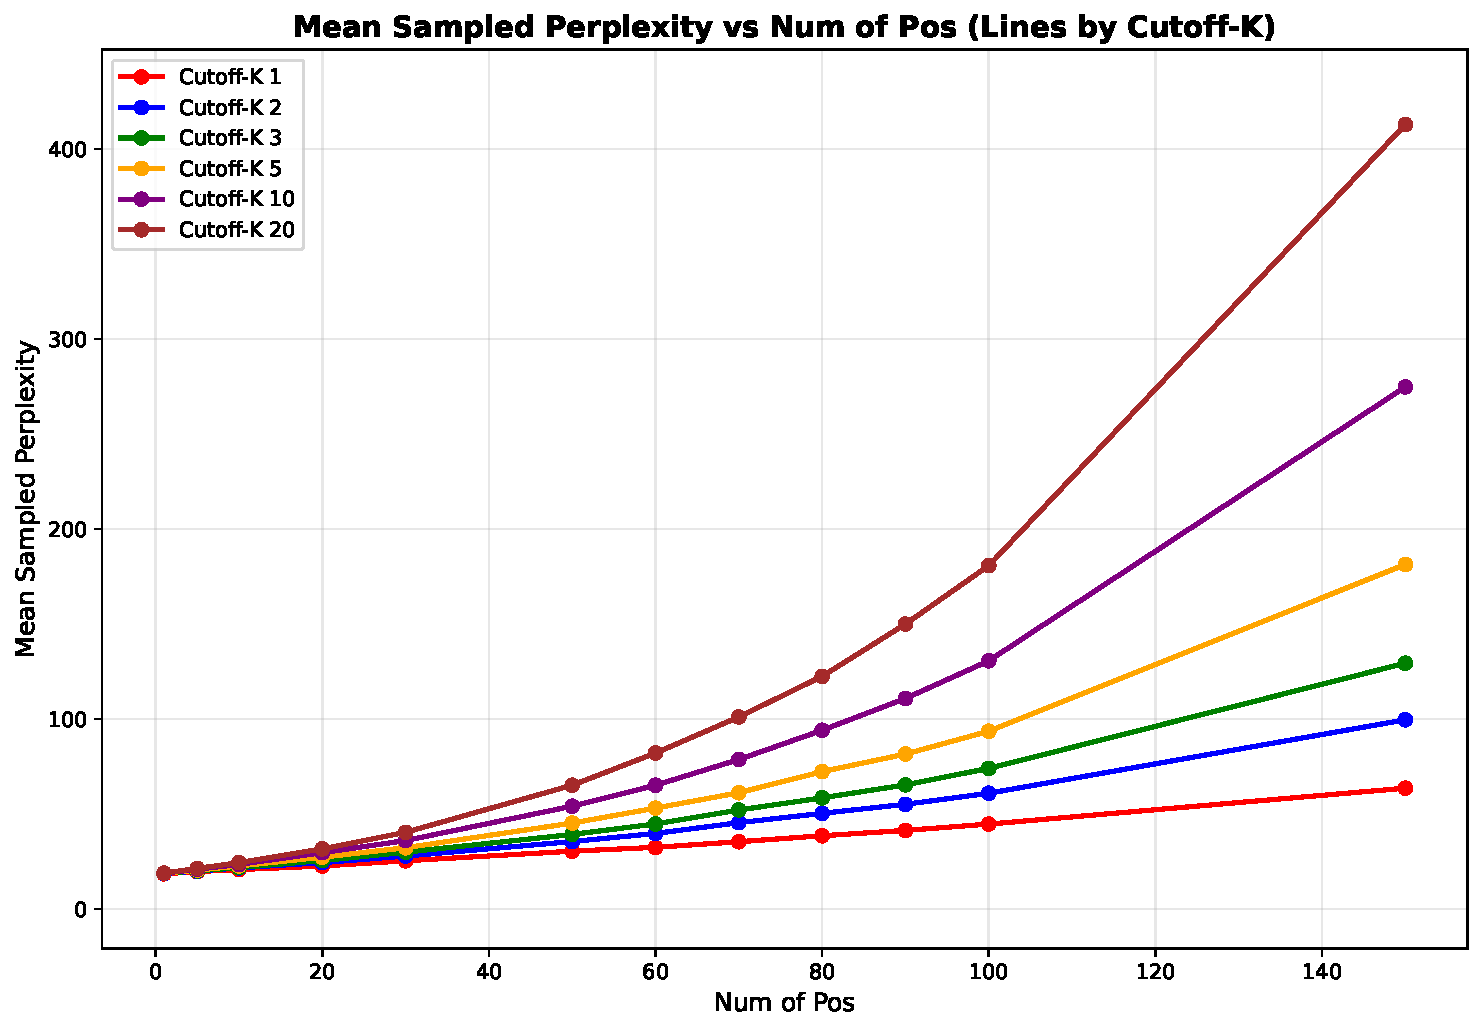
\includegraphics[width=0.45\textwidth]{graphs/attack/perplexity_main.pdf} % scale as needed
    \caption{Mean sampled perplexity vs number of perturbations made. Presented per each cutoff tested. The trend follows inverse curve to the model performance. Measured on facebook/opt-125m~\cite{facebook125m}.}
    \label{fig:perplexity}
\end{figure}

\begin{figure}[H]
    \centering
    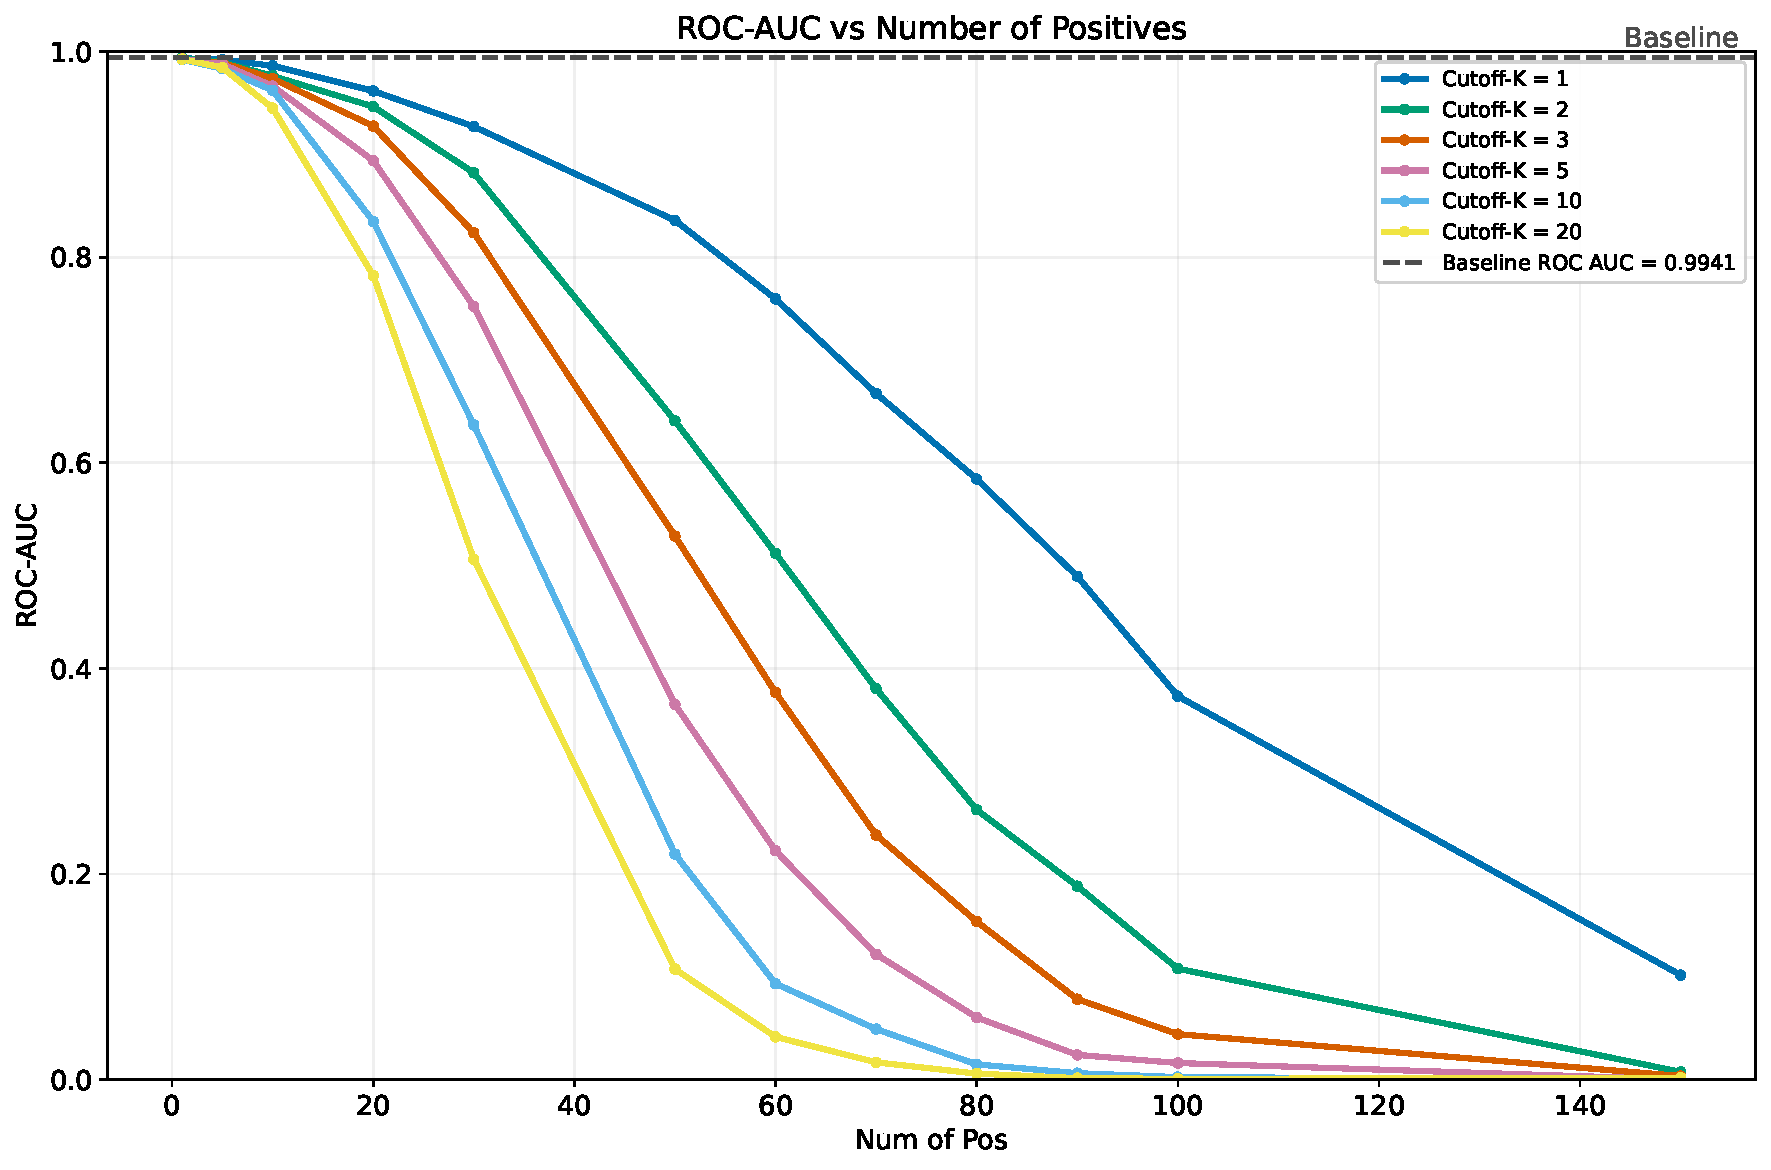
\includegraphics[width=0.45\textwidth]{graphs/attack/roc_vs_pos_by_k.pdf} % scale as needed
    \caption{AUROC vs number of perturbed positions, shown separately for different cutoff values. The dashed line indicates baseline performance without perturbation. AUROC decreases as the number of perturbations increases, with larger cutoffs accelerating the degradation. Results are reported for GPT-2 (124M)~\cite{radford2019language}.}
    \label{fig:ROC_attack}
\end{figure}

\begin{table}[H]
    \caption{Example texts under Mid-K attack with GPT-2 (124M) on XSum.}
    \label{tab:placeholder}
\vspace{1em}
\noindent
\textbf{Perturbation Results:}
\\
\begin{tabular}{|p{0.2\linewidth}|p{0.75\linewidth}|}
    \hline
    \textbf{Pos / Limit} & \textbf{Text} \\
    \hline
    Human & ``It was an oversight,'' Palmer told BBC Sport.\\
    \hline
    No perturbation & ``It was an honest and open challenge over the length of time,'' he said. \\
    \hline
    50 / 5 & ``It was an honest and open challenge over the length of time,'' he tells us.\\
    \hline
    150 / 1 & ``It was an honest and open challenge over exactly how this particular scheme could have become so costly to operate after it closed in 2001, we still do to this present day,'' said the report said\\
    \hline
    150 / 20 & ``It was an inappropriate response by the HL [Herodoplyosis Unit to complain that player Eddie Gabboni ran red before half goal]; in such situations players wear distinctive black shorts (most usually found throughout tournaments by Uprod on other social programs at venues as in RTS).\\
    \hline
\end{tabular}
\end{table}

\section{Algorithms}

\begin{algorithm*}[h]
  \caption{Fast-DetectGPT machine-generated text detection.}
  \textbf{Input:} passage $x$, sampling model $q_\varphi$, scoring model $p_\theta$, and decision threshold $\epsilon$ \\
  \textbf{Output:} True -- probably machine-generated, False -- probably human-written.
  \begin{algorithmic}[1]
    \label{alg:fastdetectgpt}
\Function{FastDetectGPT}{$x, q_\varphi, p_\theta$}
    \State $\tilde{x}_i \sim q_\varphi(\tilde{x}|x), i \in [1..N]$ \hfill $\triangleright$ Conditional sampling
    \State $\tilde{\mu} \leftarrow \frac{1}{N} \sum_i \log p_\theta(\tilde{x}_i|x)$ \hfill $\triangleright$ Estimate the mean
    \State $\tilde{\sigma}^2 \leftarrow \frac{1}{N-1} \sum_i (\log p_\theta(\tilde{x}_i|x) - \tilde{\mu})^2$ \hfill $\triangleright$ Estimate the variance
    \State $\hat{\mathrm{d}}_x \leftarrow (\log p_\theta(x) - \tilde{\mu})/\tilde{\sigma}$ \hfill $\triangleright$ Estimate conditional probability curvature
    \State \Return $\hat{\mathrm{d}}_x > \epsilon$ \hfill $\triangleright$ Compare with threshold
\EndFunction
\end{algorithmic}
\end{algorithm*}

\begin{algorithm*}[h]
  \caption{DetectGPT machine-generated text detection}
  \begin{algorithmic}[1]
    \label{alg:detectgpt}
\State \textbf{Input:} passage $x$, source model $p_\theta$, perturbation function $q$, number of perturbations $k$, decision threshold $\epsilon$
\State $\tilde{x}_i \sim q(\cdot \mid x)$, $i \in [1..k]$ \hfill $\triangleright$ mask spans, sample replacements
\State $\hat{\mu} \leftarrow \frac{1}{k} \sum_i \log p_\theta(\tilde{x}_i)$ \hfill $\triangleright$ approximate expectation in Eq. 1
\State $\hat{\mathrm{d}}_x \leftarrow \log p_\theta(x) - \hat{\mu}$ \hfill $\triangleright$ estimate d $(x, p_\theta, q)$
\State $\tilde{\sigma}_x^2 \leftarrow \frac{1}{k-1} \sum_i (\log p_\theta(\tilde{x}_i) - \hat{\mu})^2$ \hfill $\triangleright$ variance for normalization
\State \textbf{if} $\frac{\hat{\mathrm{d}}_x}{\tilde{\sigma}_x} > \epsilon$ \textbf{then}
\State \quad return \texttt{true} \hfill $\triangleright$ probably model sample
\State \textbf{else}
\State \quad return \texttt{false} \hfill $\triangleright$ probably not model sample
\end{algorithmic}
\end{algorithm*}





\end{document}